\documentclass[11pt,titlepage]{scrartcl}

% Based on thesisclass.cls of Timo Rohrberg, 2009
% ----------------------------------------------------------------
% Thesis - Main document
% ----------------------------------------------------------------
\usepackage{wrapfig}

% Set document encoding to UTF-8.
\usepackage[utf8]{inputenc}
% \usepackage[latin1]{inputenc} % Input in ISO 8859-1 (Latin1)
% Use vector glyphs of Computer Modern font with T1 encoding.
\usepackage{lmodern}
\usepackage[T1]{fontenc}
% Activate micro-typographic improvements.
\usepackage[protrusion=true,expansion=true]{microtype}
% \usepackage{ae}               % Almost european, virtual T1-Font
% Activate color definitions.
\usepackage[pdftex]{xcolor}
% Make including other pdfs available.
\usepackage[pdftex]{graphicx}
% Additional math symbols.
\usepackage{amssymb,amsmath,amsthm}
% Smart spacing for macros.
\usepackage{xspace}
% Rotated table head labels.
\usepackage{rotating}
% Nice table separator lines.
\usepackage{booktabs}

\usepackage{vmargin}          % Adjust margins in a simple way
\usepackage{fancyhdr}         % Define simple headings
\usepackage{subfigure}
\usepackage{url}
\usepackage[absolute,overlay]{textpos}
\usepackage{tikz}
\usepackage[english,ngerman]{babel}
\usepackage[ruled, vlined, linesnumbered]{algorithm2e}
\usepackage[raiselinks=true,
						bookmarks=true,
						bookmarksopenlevel=1,
						bookmarksopen=true,
						bookmarksnumbered=true,
						hyperindex=true,
						plainpages=false,
						pdfpagelabels=true,
						pdfborder={0 0 0.5},
						colorlinks=false,
						linkbordercolor={0 0.61 0.50},
						citebordercolor={0 0.61 0.50}]{hyperref}  %{0.57 0.74 0.57}

\usepackage[fixlanguage]{babelbib}	% sets german style for literature entries
\selectbiblanguage{ngerman}		% for \bibliographystyle{babalpha}

%% -------------------------------
%% |      Globale Settings       |
%% -------------------------------
\setcounter{secnumdepth}{3} % Numbering also for \subsubsections
\setcounter{tocdepth}{3}    % Register \subsubsections in content directory

\setpapersize{A4}
\setmarginsrb{3cm}{1cm}{3cm}{1cm}{6mm}{7mm}{5mm}{15mm}

\parindent 0cm                     % Do not indent beginning of paragraph
\parskip1.5ex plus0.5ex minus0.5ex % Margin between paragraphs

%% --- End of global Settings ---

%% -------------------------------
%% |  Information for PDF file   |
%% -------------------------------
\hypersetup{
 pdfauthor={?},
 pdftitle={?},
 pdfsubject={?},
 pdfkeywords={?}
}


%% ---------------------------------
%% | Information about the thesis  |
%% ---------------------------------

\title{Visualisierung von Argumentkarten - Inkrementelle Layouts}
\author{Stefan Altmayer, Lukas Barth, Eric Braun, David Hopf, Frederike Neuber}

% \newcommand{\myname}{Stefan Altmayer, Lukas Barth, Eric Braun, David Hopf, Frederike Neuber}
% \newcommand{\mytitle}{Visualisierung von Argumentkarten - Inkrementelle Layouts}
% \newcommand{\myinstitute}{Institute of Theoretical Computer Science}
%
% \newcommand{\reviewerone}{?}
% \newcommand{\reviewertwo}{?}
% \newcommand{\advisor}{Ignaz Rutter}
% \newcommand{\advisortwo}{Andreas Gemsa}
%
% \newcommand{\timestart}{1st October 2014}
% \newcommand{\timeend}{31th March 2015}


\newcommand{\NP}{\ensuremath{\mathcal{NP}}}


%% ---------------------------------
%% | Commands                      |
%% ---------------------------------

\newtheorem{definition}{Definition}
\newtheorem{theorem}[definition]{Theorem}
\newtheorem{lemma}[definition]{Lemma}
\newtheorem{corollary}[definition]{Corollary}
\newtheorem{conjecture}[definition]{Conjecture}


%% --------------------------------
%% | Settings for word separation |
%% --------------------------------
% Help for separation:
% In german package the following hints are additionally available:
% "- = Additional separation
% "| = Suppress ligation and possible separation (e.g. Schaf"|fell)
% "~ = Hyphenation without separation (e.g. bergauf und "~ab)
% "= = Hyphenation with separation before and after
% "" = Separation without a hyphenation (e.g. und/""oder)

% Describe separation hints here:
\hyphenation{
% Pro-to-koll-in-stan-zen
% Ma-na-ge-ment  Netz-werk-ele-men-ten
% Netz-werk Netz-werk-re-ser-vie-rung
% Netz-werk-adap-ter Fein-ju-stier-ung
% Da-ten-strom-spe-zi-fi-ka-tion Pa-ket-rumpf
% Kon-troll-in-stanz
}



%%%%%%%%%%%%%%%%%%%%%%%%%%%%%%%%%
%% Here, main documents begins %%
%%%%%%%%%%%%%%%%%%%%%%%%%%%%%%%%%
\begin{document}

% Remove the following line for German text
%\selectlanguage{english}

\pagenumbering{roman}
\maketitle


%% -------------------
%% |   Abstract      |
%% -------------------

% \thispagestyle{plain}
%
% \begin{addmargin}{0.5cm}
%
% \centerline{\bf Abstract}
%
% A short summary of what is going on here.
%
% \vskip 2cm
%
% \centerline{\bf Deutsche Zusammenfassung}
%
% Kurze Inhaltsangabe auf deutsch.
%
% \end{addmargin}

%% -----------------
%% |   Main part   |
%% -----------------

\pagenumbering{arabic}
%%% introduction.tex
%%
\label{sub:intro}

In dieser Arbeit beschäftigen wir uns mit der Frage, wie Argumentkarten inkrementell gelayoutet werden können. Argumentkarten sind Hilfsmittel, um komplexe Argumentationen oder Debatten darzustellen. Die Knoten in einem solchen Graphen stellen Sätze oder einzelne Thesen dar; die Kanten zeigen Beziehungen an - sie stützen andere Thesen oder Argumente, oder greifen diese an.
 Da Argumentkarten oft die Funktion haben, eine bestehende Debatte oder einen Text abzubilden, oder ein Werkzeug bei der Strukturierung derselben sein sollen, kann es gewünscht sein, dass die Struktur der Karte wichtige Aspekte der Struktur des Vorbildes erkennen lässt: So kann es beispielsweise sein, dass die Leserichtung der Karte - also von links oben nach rechts unten - der Abfolge der entsprechenden Thesen und Argumente in einer vorhandenen Debatte oder einem Text entsprechen soll. Es kann auch sein, dass eine Reihe von zusammengehörigen Argumenten nummeriert wird, um ihre Abfolge in der zu repräsentierenden Argumentation anzuzeigen. Auch ist vorstellbar, dass die spezifische Anordnung von einigen Knoten weitere Informationen vermitteln sollen - etwa, dass diese die zentralen Thesen des Textes sind oder zwischen jenen Argumenten der zentrale Konflikt der Debatte stattfindet, dem sich die anderen Thesen und Argumente jeweils unterordnen lassen

Abstrakt betrachtet sind Argumentkarten gelayoutete Graphen, bei denen Knoten nicht punktförmig, sondern durch Rechtecke repräsentiert werden.

Das Problem des inkrementellen Layouts besteht darin, eine bereits existierende Argumentkarte zu verändern und für diese veränderte Argumentkarte ein neues Layout zu finden. Das neue Layout soll dabei in einer Weise gefunden werden, die die "`mentale Karte"' erhält, dass also ein menschlicher Betrachter, der die alte Karte kannte, sich in der neuen Karte schnell zurecht findet. Dies erreichen wir, indem wir die neue Karte so layouten, dass sie der alten, bekannten Karte ähnlich ist.

Wir haben uns außerdem dafür entschieden, als Veränderungen der Karte ausschließlich das Hinzufügen eines einzelnen Knotens zu betrachten. Die Entfernung einer kleinen Anzahl von Knoten ist vermutlich gut durch einfaches Weglassen der Knoten umsetzbar, und daher algorithmisch nicht interessant. Die meisten anderen Operationen, wie zum Beispiel das Verschieben von Knoten, können dann als eine Aufeinanderfolge von Entfernungs- und Einfügeoperationen dargestellt werden.

In dieser Arbeit werden wir nun zunächst eine Formalisierung dieses Problems vorstellen, um dann zwei Ideen für heuristische Lösungsmöglichkeiten zu präsentieren. Danach werden wir einige Integer Linear Programs vorstellen, die das Problem unserer Meinung nach besser lösen als die angedachten Heuristiken. Abschließend präsentieren wir einige Implementation eines solchen ILPs.

\subsection{Besondere Anforderungen}
\label{sub:tasks}

Für die vorliegende Arbeit ist nun besonders interessant, dass eine Argumentkarte, einmal vom Ersteller nach den oben genannten Gesichtspunkten in ein ansprechendes Layout gebracht, oft nicht in dieser Form bestehen bleibt. Argumentkarten werden in verschiedenen Versionen präsentiert, nach Diskussion überarbeitet oder verändern sich - etwa bei der Rekonstruktion laufender Debatten oder begleitend zu einem in der Entstehung befindlichen Text - sogar ständig weiter. Diese Umstände verlangen einen Layout-Algorithmus mit besondere Anforderungen: Zum Einen soll er natürlich in der Lage sein, inkrementell hinzugefügte Elemente in der Karte ästhetisch ansprechend in der bestehenden Karte unterzubringen. Zum Anderen soll die so entstandene, neue Karte aber der alten Version hinreichend ähnlich sehen, damit die oben genannten Möglichkeiten, die Struktur von Debatten oder Argumentationen mit Hilfe der Argumentkarte darzustellen, nicht verloren gehen.

 So könnte es passieren, dass die Reihenfolge der Knoten sich durch die Einfügung eines einzelnen Elements massiv ändert, um Platz zu schaffen - und auch die Leserichtung nicht mehr mit beispielsweise einem Ursprungstext übereinstimmt. Auch wenn der Benutzer eine Reihe von Knoten manuell nummeriert und hierarchisch geordnet hat, um zusammengehörige Elemente anzuzeigen, kann es passieren, dass die entsprechenden Knoten durch ein erneutes Layouten plötzlich in falscher Reihenfolge angeordnet werden. Die Intention, die der Benutzer bei der Anordnung gezielt ausgewählter Knoten verfolgte, kann nicht mehr erkennbar sein, weil bei einem neuen Layout wichtige Merkmale, wie die Abstände und wechselseitige Ausrichtung dieser Knoten sich geändert hat, um ein neues Element in der Karte unterbringen zu können.

 Ein Layout-Algorithmus, der diese Probleme vermeidet und die genannten Strukturierungsmöglichkeiten auch bei inkrementellem Layout mit laufend hinzukommenden, neuen Elementen beibehält, wäre für die Erstellung von Argumentkarten daher äußerst wünschenswert.

%% ==============================
\subsection{Das Problem}
\label{sub:problem}
%% ==============================

Das Problem stellt sich aus Sicht eines Informatikers wie folgt dar. Gegeben sind:

\begin{enumerate}
  \item ein Graph $G = (V, E)$
  \item je ein Rechteck pro Knoten, oder genauer eine Funktion $b: V \rightarrow R^2$, die jedem Knoten seine Höhe und Breite zuordnet,
  \item eine (überlappungsfreie) geometrische Einbettung von $G$, also eine Funktion $\omega: V \rightarrow R^2$, die jedem Knoten einen Punkt in der Ebene zuweist,
  \item ein einzufügender neuer Knoten $a \in R^2$ mit einer Menge $M$ von Knoten, zu denen er adjazent ist
  \item eine Funktion $\psi: M \rightarrow R^2$, die zu jedem Knoten $m \in M$ adjazent zu $a$ den Vektor zuordnet, der angibt, wie $a$ relativ zu $m$ platziert werden soll.
\end{enumerate}

Gesucht ist dann eine neue geometrische Einbettung $\omega'$ von $(V \cup \{a\}, E \cup \{(a,m) \mid m \in M\}$, die "`ähnlich"' ist zu $\omega$.

\begin{paragraph}{Ähnlichkeit}
  Bei der Definition der zu optimierenden Ähnlichkeit bieten sich mehrere Ansätze an: Zunächst die \textit{absolute Ähnlichkeit}, bei der schlicht die Summe der Entfernungen aller Positionen von ihren Ursprungspositionen minimiert wird, also
  \begin{equation}
    \min_{\omega'} \sum \limits_{v \in V} {|\omega(v) - \omega'(v)|}
  \end{equation}

  Diese Definition erschien uns jedoch zu starr. Insbesondere sind wir der Meinung, dass der Erhalt der "`mentalen Karte"' hauptsächlich davon abhängig ist, wie die Positionen der Knoten zueinander sind. Ein in unseren Augen besserer Ansatz könnte also lauten:
  \begin{equation}
    \min_{\omega'} \sum \limits_{(v,w) \in V \times V} {|(\omega(v) - \omega(w)) - (\omega'(v) - \omega'(w))|}
  \end{equation}

  Aber auch hier geht in die Optimierung noch die relative Position von zwei Knoten ein, die vielleicht an ganz unterschiedlichen Enden der Argumentkarte stehen, und bei denen eine Abweichung von der gewünschten relativen Position weniger stört als bei zwei Knoten, die dicht beieinander, und somit vermutlich auch in einem engeren semantischen Zusammenhang stehen. Dies könnte man nun über Gewichtungen versuchen zu lösen, wir haben uns aber entschieden, stattdessen nur die relativen Positionen von adjazenten Knoten zu betrachten:
  \begin{equation}
    \label{eqn:opt:basic}
    \min_{\omega'} \sum \limits_{(v,w) \in E} {|(\omega(v) - \omega(w)) - (\omega'(v) - \omega'(w))|}
  \end{equation}
\end{paragraph}

Zusätzlich muss noch die Position des neu einzufügenden Knotens berücksichtigt werden. Wäre nicht angegeben, wie der neue Knoten relativ zu seinen Nachbarn positioniert werden soll, so würde er vermutlich einfach außerhalb der bisher gelayouteten Argumentkarte platziert, da so der Term \ref{eqn:opt:basic} durch die alten Positionen optimiert wird, ohne dass eine Überlappung entstehen würde. Wir fügen also hinzu:

\begin{equation}
  \label{eqn:opt:new}
  \min_{\omega'} \sum \limits_{m \in M} {|(\psi(m)) - (\omega'(a) - \omega'(m))|}
\end{equation}

\begin{paragraph}{Verschiebung versus Skalierung}
  \label{par:scale}
  Wenn wir für einen Moment davon ausgehen, dass das neue Layout nicht überlappungsfrei sein muss, so werden (eine geeignete Wahl von $\psi$ vorausgesetzt) die Summen \ref{eqn:opt:new} und \ref{eqn:opt:basic} (zu Null) dadurch optimiert, dass alle alten Knoten auf ihren Plätzen bleiben und der neue Knoten am gewünschten Punkt (mit alten Knoten überlappend) eingefügt wird. Ausgehend von diesem Layout sehen wir zwei grundlegend verschiedene Möglichkeiten, den notwendigen Platz für ein überlappungsfreies Layout zu schaffen: Zunächst können natürlich einfach einzelne Knoten verschoben werden. Dies "`verzerrt"' die relativen Positionen von Knoten und erhöht die Summen \ref{eqn:opt:new} und \ref{eqn:opt:basic}. Andererseits ist es aber auch möglich, einfach alle Kantenlängen mit einem gewissen Faktor zu multiplizieren, was dadurch, dass das Layout insgesamt größer wird, äquivalent dazu ist, die Knotengrößen kleiner zu skalieren. Diese zweite Möglichkeit erhöht ebenfalls beide Summen, wir sind allerdings der Meinung, dass dies nicht der Fall sein sollte: Für den Betrachter ändert sich nicht die relative Lage der Knoten zueinander, die Knoten werden nur kleiner. Wir führen daher einen Skalierungsfaktor $c$ ein. Natürlich muss $c$ so gewählt werden, dass er möglichst nah an $1$ gelegen ist. Insgesamt ergibt sich somit als Optimierungsfunktion:
\end{paragraph}

\begin{align}
  \label{eqn:opt:complete}
 \min_{\omega'} \quad & \alpha \sum \limits_{(v,w) \in E} {|c(\omega(v) - \omega(w)) - (\omega'(v) - \omega'(w))|} \nonumber \\
  + & \beta \sum \limits_{m \in M} {|(c\psi(m)) - (\omega'(a) - \omega'(m))|} \nonumber \\
  + & \gamma (|1 - c|)
\end{align}

Zeilen $1$ und $2$ entsprechen dabei den Summen \ref{eqn:opt:new} und \ref{eqn:opt:basic} unter Berücksichtigung von $c$. Die Koeffizienten $\alpha, \beta$ und $\gamma$ dienen dazu, die einzelnen Teile der Optimierungsfunktion gegeneinander zu gewichten.

%%% preliminaries.tex
%%

%% ==============
\chapter{Preliminaries}
\label{ch:preliminaries}
%% ==============

This chapter should provide the foundations of the thesis.
%% content.tex
%%

%% ==============
%\chapter{Content Chapters}
\label{ch:Content1}
%% ==============

\section{Einführung}

%% introduction.tex
%%
\label{sub:intro}

In dieser Arbeit beschäftigen wir uns mit der Frage, wie Argumentkarten inkrementell gelayoutet werden können. Argumentkarten sind Hilfsmittel, um komplexe Argumentationen oder Debatten darzustellen. Die Knoten in einem solchen Graphen stellen Sätze oder einzelne Thesen dar; die Kanten zeigen Beziehungen an - sie stützen andere Thesen oder Argumente, oder greifen diese an.
 Da Argumentkarten oft die Funktion haben, eine bestehende Debatte oder einen Text abzubilden, oder ein Werkzeug bei der Strukturierung derselben sein sollen, kann es gewünscht sein, dass die Struktur der Karte wichtige Aspekte der Struktur des Vorbildes erkennen lässt: So kann es beispielsweise sein, dass die Leserichtung der Karte - also von links oben nach rechts unten - der Abfolge der entsprechenden Thesen und Argumente in einer vorhandenen Debatte oder einem Text entsprechen soll. Es kann auch sein, dass eine Reihe von zusammengehörigen Argumenten nummeriert wird, um ihre Abfolge in der zu repräsentierenden Argumentation anzuzeigen. Auch ist vorstellbar, dass die spezifische Anordnung von einigen Knoten weitere Informationen vermitteln sollen - etwa, dass diese die zentralen Thesen des Textes sind oder zwischen jenen Argumenten der zentrale Konflikt der Debatte stattfindet, dem sich die anderen Thesen und Argumente jeweils unterordnen lassen

Abstrakt betrachtet sind Argumentkarten gelayoutete Graphen, bei denen Knoten nicht punktförmig, sondern durch Rechtecke repräsentiert werden.

Das Problem des inkrementellen Layouts besteht darin, eine bereits existierende Argumentkarte zu verändern und für diese veränderte Argumentkarte ein neues Layout zu finden. Das neue Layout soll dabei in einer Weise gefunden werden, die die "`mentale Karte"' erhält, dass also ein menschlicher Betrachter, der die alte Karte kannte, sich in der neuen Karte schnell zurecht findet. Dies erreichen wir, indem wir die neue Karte so layouten, dass sie der alten, bekannten Karte ähnlich ist.

Wir haben uns außerdem dafür entschieden, als Veränderungen der Karte ausschließlich das Hinzufügen eines einzelnen Knotens zu betrachten. Die Entfernung einer kleinen Anzahl von Knoten ist vermutlich gut durch einfaches Weglassen der Knoten umsetzbar, und daher algorithmisch nicht interessant. Die meisten anderen Operationen, wie zum Beispiel das Verschieben von Knoten, können dann als eine Aufeinanderfolge von Entfernungs- und Einfügeoperationen dargestellt werden.

In dieser Arbeit werden wir nun zunächst eine Formalisierung dieses Problems vorstellen, um dann zwei Ideen für heuristische Lösungsmöglichkeiten zu präsentieren. Danach werden wir einige Integer Linear Programs vorstellen, die das Problem unserer Meinung nach besser lösen als die angedachten Heuristiken. Abschließend präsentieren wir einige Implementation eines solchen ILPs.

\subsection{Besondere Anforderungen}
\label{sub:tasks}

Für die vorliegende Arbeit ist nun besonders interessant, dass eine Argumentkarte, einmal vom Ersteller nach den oben genannten Gesichtspunkten in ein ansprechendes Layout gebracht, oft nicht in dieser Form bestehen bleibt. Argumentkarten werden in verschiedenen Versionen präsentiert, nach Diskussion überarbeitet oder verändern sich - etwa bei der Rekonstruktion laufender Debatten oder begleitend zu einem in der Entstehung befindlichen Text - sogar ständig weiter. Diese Umstände verlangen einen Layout-Algorithmus mit besondere Anforderungen: Zum Einen soll er natürlich in der Lage sein, inkrementell hinzugefügte Elemente in der Karte ästhetisch ansprechend in der bestehenden Karte unterzubringen. Zum Anderen soll die so entstandene, neue Karte aber der alten Version hinreichend ähnlich sehen, damit die oben genannten Möglichkeiten, die Struktur von Debatten oder Argumentationen mit Hilfe der Argumentkarte darzustellen, nicht verloren gehen.

 So könnte es passieren, dass die Reihenfolge der Knoten sich durch die Einfügung eines einzelnen Elements massiv ändert, um Platz zu schaffen - und auch die Leserichtung nicht mehr mit beispielsweise einem Ursprungstext übereinstimmt. Auch wenn der Benutzer eine Reihe von Knoten manuell nummeriert und hierarchisch geordnet hat, um zusammengehörige Elemente anzuzeigen, kann es passieren, dass die entsprechenden Knoten durch ein erneutes Layouten plötzlich in falscher Reihenfolge angeordnet werden. Die Intention, die der Benutzer bei der Anordnung gezielt ausgewählter Knoten verfolgte, kann nicht mehr erkennbar sein, weil bei einem neuen Layout wichtige Merkmale, wie die Abstände und wechselseitige Ausrichtung dieser Knoten sich geändert hat, um ein neues Element in der Karte unterbringen zu können.

 Ein Layout-Algorithmus, der diese Probleme vermeidet und die genannten Strukturierungsmöglichkeiten auch bei inkrementellem Layout mit laufend hinzukommenden, neuen Elementen beibehält, wäre für die Erstellung von Argumentkarten daher äußerst wünschenswert.

%% ==============================
\subsection{Das Problem}
\label{sub:problem}
%% ==============================

Das Problem stellt sich aus Sicht eines Informatikers wie folgt dar. Gegeben sind:

\begin{enumerate}
  \item ein Graph $G = (V, E)$
  \item je ein Rechteck pro Knoten, oder genauer eine Funktion $b: V \rightarrow R^2$, die jedem Knoten seine Höhe und Breite zuordnet,
  \item eine (überlappungsfreie) geometrische Einbettung von $G$, also eine Funktion $\omega: V \rightarrow R^2$, die jedem Knoten einen Punkt in der Ebene zuweist,
  \item ein einzufügender neuer Knoten $a \in R^2$ mit einer Menge $M$ von Knoten, zu denen er adjazent ist
  \item eine Funktion $\psi: M \rightarrow R^2$, die zu jedem Knoten $m \in M$ adjazent zu $a$ den Vektor zuordnet, der angibt, wie $a$ relativ zu $m$ platziert werden soll.
\end{enumerate}

Gesucht ist dann eine neue geometrische Einbettung $\omega'$ von $(V \cup \{a\}, E \cup \{(a,m) \mid m \in M\}$, die "`ähnlich"' ist zu $\omega$.

\begin{paragraph}{Ähnlichkeit}
  Bei der Definition der zu optimierenden Ähnlichkeit bieten sich mehrere Ansätze an: Zunächst die \textit{absolute Ähnlichkeit}, bei der schlicht die Summe der Entfernungen aller Positionen von ihren Ursprungspositionen minimiert wird, also
  \begin{equation}
    \min_{\omega'} \sum \limits_{v \in V} {|\omega(v) - \omega'(v)|}
  \end{equation}

  Diese Definition erschien uns jedoch zu starr. Insbesondere sind wir der Meinung, dass der Erhalt der "`mentalen Karte"' hauptsächlich davon abhängig ist, wie die Positionen der Knoten zueinander sind. Ein in unseren Augen besserer Ansatz könnte also lauten:
  \begin{equation}
    \min_{\omega'} \sum \limits_{(v,w) \in V \times V} {|(\omega(v) - \omega(w)) - (\omega'(v) - \omega'(w))|}
  \end{equation}

  Aber auch hier geht in die Optimierung noch die relative Position von zwei Knoten ein, die vielleicht an ganz unterschiedlichen Enden der Argumentkarte stehen, und bei denen eine Abweichung von der gewünschten relativen Position weniger stört als bei zwei Knoten, die dicht beieinander, und somit vermutlich auch in einem engeren semantischen Zusammenhang stehen. Dies könnte man nun über Gewichtungen versuchen zu lösen, wir haben uns aber entschieden, stattdessen nur die relativen Positionen von adjazenten Knoten zu betrachten:
  \begin{equation}
    \label{eqn:opt:basic}
    \min_{\omega'} \sum \limits_{(v,w) \in E} {|(\omega(v) - \omega(w)) - (\omega'(v) - \omega'(w))|}
  \end{equation}
\end{paragraph}

Zusätzlich muss noch die Position des neu einzufügenden Knotens berücksichtigt werden. Wäre nicht angegeben, wie der neue Knoten relativ zu seinen Nachbarn positioniert werden soll, so würde er vermutlich einfach außerhalb der bisher gelayouteten Argumentkarte platziert, da so der Term \ref{eqn:opt:basic} durch die alten Positionen optimiert wird, ohne dass eine Überlappung entstehen würde. Wir fügen also hinzu:

\begin{equation}
  \label{eqn:opt:new}
  \min_{\omega'} \sum \limits_{m \in M} {|(\psi(m)) - (\omega'(a) - \omega'(m))|}
\end{equation}

\begin{paragraph}{Verschiebung versus Skalierung}
  \label{par:scale}
  Wenn wir für einen Moment davon ausgehen, dass das neue Layout nicht überlappungsfrei sein muss, so werden (eine geeignete Wahl von $\psi$ vorausgesetzt) die Summen \ref{eqn:opt:new} und \ref{eqn:opt:basic} (zu Null) dadurch optimiert, dass alle alten Knoten auf ihren Plätzen bleiben und der neue Knoten am gewünschten Punkt (mit alten Knoten überlappend) eingefügt wird. Ausgehend von diesem Layout sehen wir zwei grundlegend verschiedene Möglichkeiten, den notwendigen Platz für ein überlappungsfreies Layout zu schaffen: Zunächst können natürlich einfach einzelne Knoten verschoben werden. Dies "`verzerrt"' die relativen Positionen von Knoten und erhöht die Summen \ref{eqn:opt:new} und \ref{eqn:opt:basic}. Andererseits ist es aber auch möglich, einfach alle Kantenlängen mit einem gewissen Faktor zu multiplizieren, was dadurch, dass das Layout insgesamt größer wird, äquivalent dazu ist, die Knotengrößen kleiner zu skalieren. Diese zweite Möglichkeit erhöht ebenfalls beide Summen, wir sind allerdings der Meinung, dass dies nicht der Fall sein sollte: Für den Betrachter ändert sich nicht die relative Lage der Knoten zueinander, die Knoten werden nur kleiner. Wir führen daher einen Skalierungsfaktor $c$ ein. Natürlich muss $c$ so gewählt werden, dass er möglichst nah an $1$ gelegen ist. Insgesamt ergibt sich somit als Optimierungsfunktion:
\end{paragraph}

\begin{align}
  \label{eqn:opt:complete}
 \min_{\omega'} \quad & \alpha \sum \limits_{(v,w) \in E} {|c(\omega(v) - \omega(w)) - (\omega'(v) - \omega'(w))|} \nonumber \\
  + & \beta \sum \limits_{m \in M} {|(c\psi(m)) - (\omega'(a) - \omega'(m))|} \nonumber \\
  + & \gamma (|1 - c|)
\end{align}

Zeilen $1$ und $2$ entsprechen dabei den Summen \ref{eqn:opt:new} und \ref{eqn:opt:basic} unter Berücksichtigung von $c$. Die Koeffizienten $\alpha, \beta$ und $\gamma$ dienen dazu, die einzelnen Teile der Optimierungsfunktion gegeneinander zu gewichten.


\section{Heuristische Ansätze}

TODO Heuristik-Blah

\subsection{Spring Embedder}

Spring Embedder sind eine Familie von Algorithmen zum Zeichnen von Graphen. Diese Algorithmen basieren im Allgemeinen darauf, dass ein physikalisches Modell simuliert wird, bei dem Kräfte auf die einzelnen Knoten wirken, die diese verschieben. Spring Embedder sind weit verbreitet, gut verstanden und recht flexibel\cite{kobourov2012spring}, sodass es naheliegend ist, diese als Möglichkeit in Betracht zu ziehen.

Wenn wir davon ausgehen, dass im gelayouteten Graphen nur die Kantenlängen (und nicht die Richtung der Kanten) das Layout bestimmen, dann ist der Term \ref{eqn:opt:basic} trivial in einen Spring Embedder umzusetzen. Dies wäre insbesondere geeignet, falls der Graph eine hohe Steifigkeit aufweist, da in diesem Fall die Kantenlängen allein das Layout des Graphen festlegen.\footnote{Dies ist nicht ganz korrekt: Es können mehrere unterschiedliche geometrische Einbettungen mit denselben Kantenlängen existieren, z.B. indem Dreiecke umgeklappt werden. Da ein Spring Embedder allerdings nur kleine, inkrementelle Änderungen der Einbettung vornimmt, ist dies hier nicht relevant.}

\begin{figure}
	\centering
	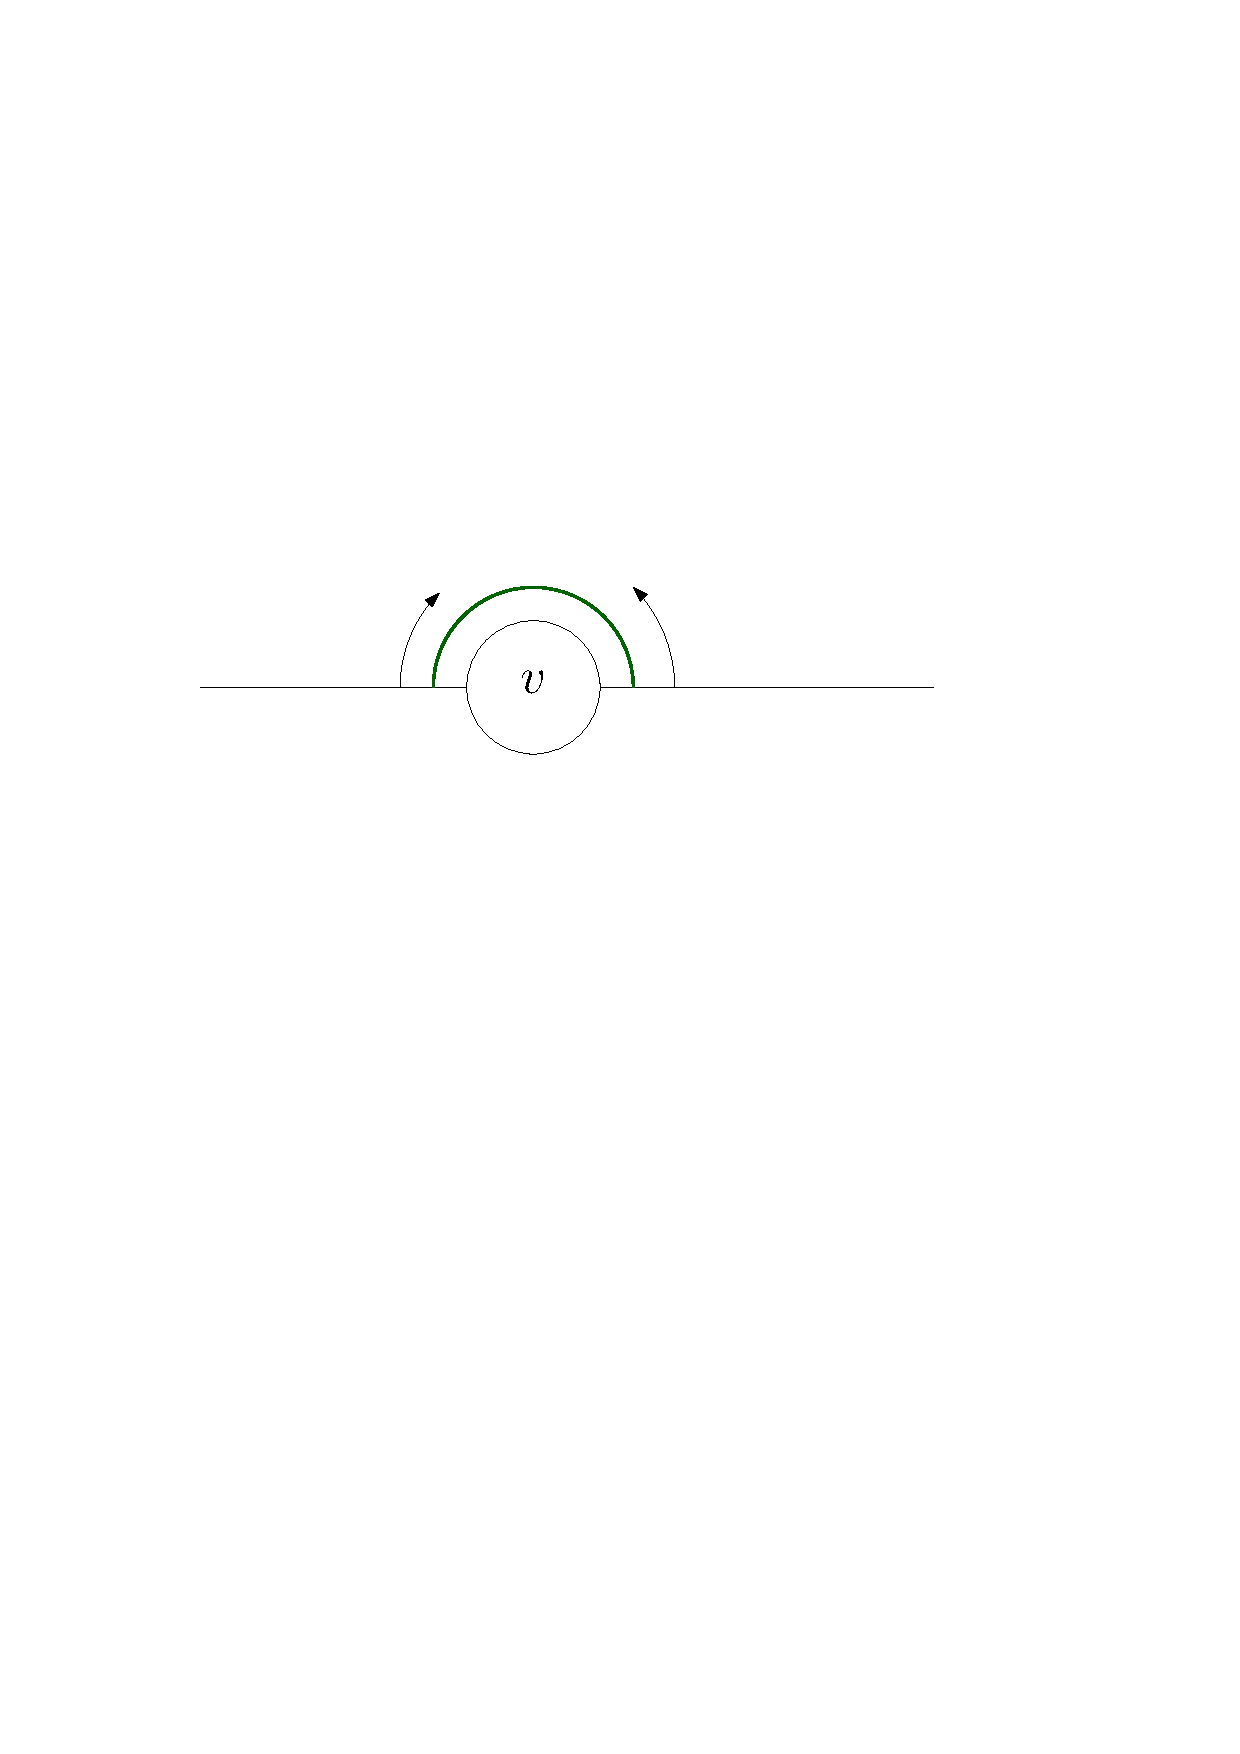
\includegraphics{figures/orbitalspring.pdf}
	\caption{Eine orbitale Feder}
	\label{fig:orbitalspring}
\end{figure}

Leider sind Argumentkarten vergleichsweise dünn besetzte Graphen, und daher ist eine geringe Steifigkeit anzunehmen. Um hier zu dem von Term \ref{eqn:opt:basic} gewünschten Ergebnis zu kommen, wäre es vermutlich notwendig, zusätzlich orbitale Federn um die Knoten herum zu legen, die die Winkel der ausgehenden Kanten relativ zueinander an das gewünschte Ergebnis anzunähern. Siehe Abbildung \ref{fig:orbitalspring}. Hier zieht die grüne kreisförmige Feder die beiden aus $v$ ausgehenden Kanten zusammen. Solche kreisförmigen Federn sind beispielsweise bereits erfolgreich für Lombardi-Zeichnungen mit optimaler Winkelauflösung verwendet worden\cite{chernobelskiy2012force}, wobei hier die Kräfte den kompletten Knoten rotiert haben, statt Auswirkungen auf die adjazenten Knoten zu haben. Kreisförmige Federn zischen Kantenpaaren konnten wir in der Literatur bisher keine finden. TODO nochmal überprüfen!

\subsection{Seam Carving}

Seam Carving ist eine verbreitete Methode in der Bildbearbeitung, die von S. Avidan und A. Shamir vorgestellt wurde.\cite{avidan2007seam} Das Ziel von Seam Carving ist es, ein Bild zu verkleinern, indem Pixel weggelassen werden, ohne visuell den Eindruck einer Verzerrung zu erwecken. Hierfür verwendet Seam Carving eine Technik, die die Autoren als "`content aware"' bezeichnen: Die wegzulassenden Pixel werden als durchgänginge Streifen, die sogenannten "`Seams"', gewählt. Bei der Auswahl der Seams wird darauf geachtet, dass diese möglichst wenig durch Bereiche des Bildes verlaufen, in denen ein Weglassen störend wäre. Hierfür beschreiben die Autoren verschiedene Energiefunktionen auf den Bildern.

\begin{figure}
	\centering
	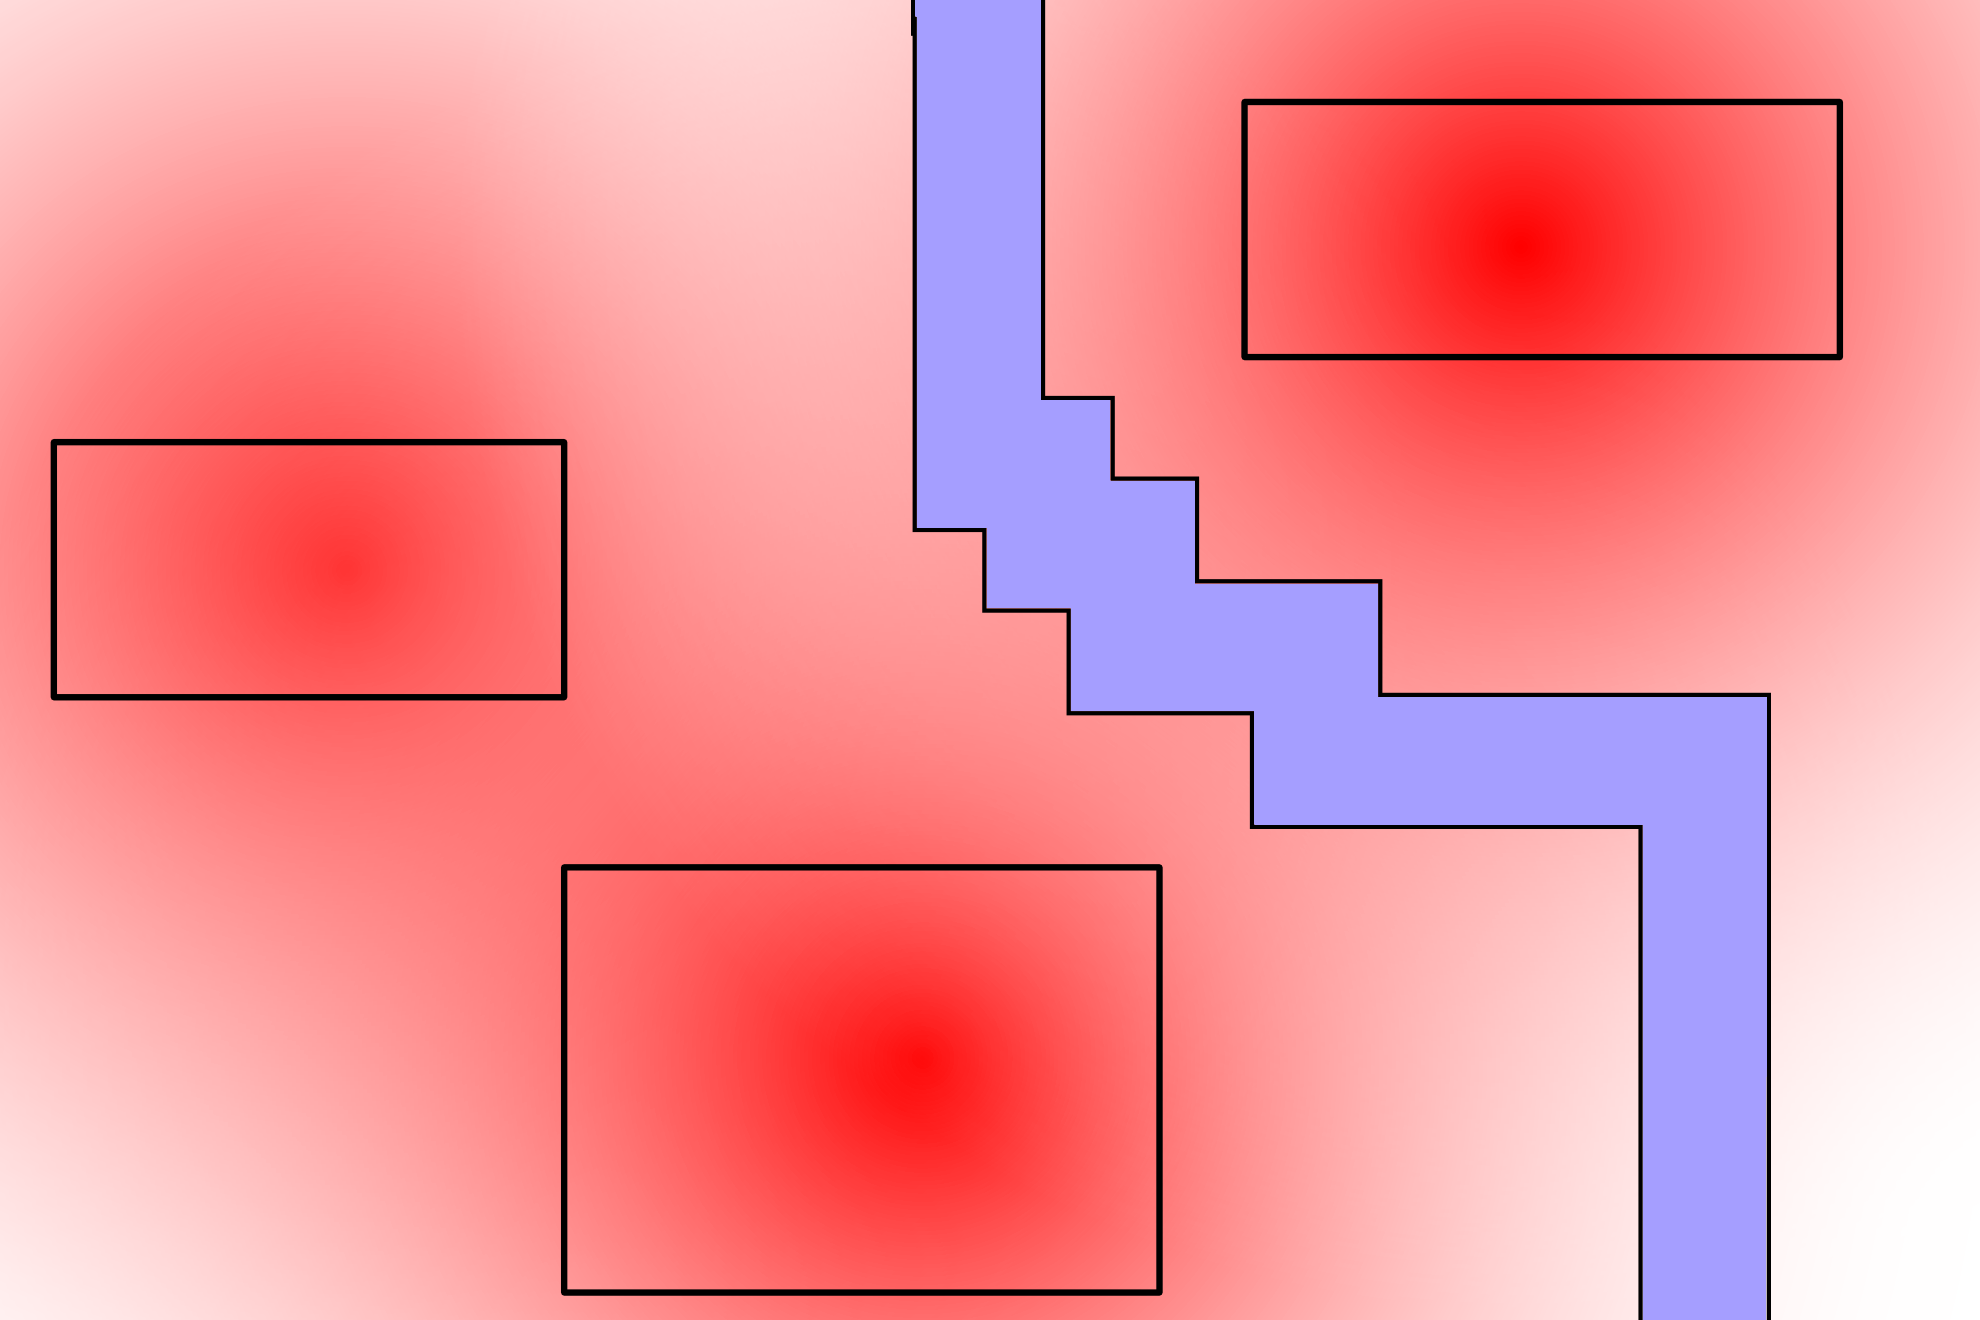
\includegraphics{figures/seamcarving.png}
	\caption{Seam Carving}
	\label{fig:seamcarving}
\end{figure}

Seam Carving hat außerdem bereits Anwendung im Bereich des Graph Drawings gefunden, beispielsweise beim Layout von Word Clouds.\cite{wu2011semantic} Das Vorgehen war hier das folgende: Ein initiales Layout verteilt die Knoten des Graphens mittels Multidimensional Scalings nach bestimmten vorgegbenen Abständen voneinander. Der überflüssige Platz wird dann mit Seam Carving entfernt. Hierbei sollten die relativen Positionen der Knoten möglichst wenig verzerrt werden. Die Autoren beschreiben hierfür die für das Seam Carving verwendete Energiefunktion als Summe der Quadrate der inversen Abstände von den Knoten. In Abbildung \ref{fig:seamcarving} ist eine solche Zeichnung mit den Energiefunktionen und einem möglichen Seam dargestellt.

Ein ähnlicher Ansatz ist auch für unser Problem denkbar. Wie in Absatz \ref{sub:problem} beschrieben, ist es immer möglich, alle Kanten einfach so lange zu skalieren, bis der neue Knoten überlappungsfrei platziert werden kann. TODO Paragraph referenzieren? Das Problem besteht hier darin, dass das gesamte Layout hierbei beliebig groß werden kann, zur Betrachtung also das Bild insgesamt verkleinert werden muss, was einer Skalierung der Knotergrößen gleichkommt. Dieses Problem könnte dadurch angegangen werden, dass das in \cite{wu2011semantic} beschriebene Verfahren ohne große Änderungen auf das Layout nach der Skalierung angewendet wird.


\section{Ein Integer Linear Program}

Die in Abschnitt \ref{sub:problem} vorgestellte formale Definition des Problems versetzt uns in die Lage, vergleichsweise einfach ein Integer Linear Program anzugeben, das die gegebene Zielfunktion optimiert. Drei Variationen wollen wir im Folgenden vorstellen.

Allgemein haben wir uns entschieden, Kanten in diesen Modellen nicht zu berücksichtigen. Wir gehen davon aus, dass es möglich ist, bei ähnlichen Knotenpositionierungen auch ein ähnliches Kantenrouting zu finden. Dies wird vermutlich insbesondere dann einfacher, wenn die Kanten auch ursprünglich algorithmisch (und nicht manuell) geroutet worden sind. Für eine erste Idee, wie das Kantenrouting behandelt werden könnte, siehe Abschnitt \ref{sub:edgeroute}.

\subsection{Statische Reihenfolge}

Wir haben uns entschieden, neben der in \ref{eqn:opt:complete} formulierten Optimierungsfunktion noch etwas schärfere Maßstäbe anzulegen, und die horizontale und vertikale Reihenfolge der Knoten jedenfalls annähernd zu fixieren. Dies ergibt sich vor allem auch aus den in Abschnitt \ref{sub:tasks} gestellten Anforderungen. Als (horizontale oder vertikale) \textit{Reihenfolge} werden wir im Folgenden immer die Ordnung der Knoten entlang ihrer $x$- oder $y$-Koordinaten verstehen. Wir nennen zwei Knoten \textit{benachbart}, wenn sie in einer dieser Reihenfolgen aufeinander folgen.

Legt man sich fest, diese Reihenfolgen beim Finden eines neuen Layouts tatsächlich nicht zu verändern, und ist außerdem vorgegeben, an welcher Stelle der neue Knoten jeweils in die Reihenfolgen einzufügen ist, so lässt sich sogar ein Lineares Programm formulieren, das \ref{eqn:opt:complete} unter dieser Bedingung optimiert.\footnote{Andernfalls ist dies nicht möglich: Wenn es erlaubt ist, Knoten $A$ links oder rechts von $B$ zu platzieren, so ist die Bedingung zur Überlappungsfreiheit nicht ohne eine Integer-Variable zu formulieren.} Dieses LP hat nur eine Art von Nebenbedingungen, nämlich die, die für jedes Paar von (geometrisch) benachbarten Knoten die Überlappungsfreiheit sicherstellt. Dies ist eine starke Einschränkung: Prinzipiell ist es in einer gültigen Zeichnung erlaubt, dass zwei Knoten sich entweder horizontal oder vertikal überlappen, nicht jedoch beides. Im Linearen Programm muss nun festgelegt werden, in welcher Dimension zwei (benachbarte) Knoten sich nicht überlappen dürfen. Eine Formulierung "`Entweder horizontal oder vertikal"' ist ohne Integer-Variablen nicht möglich. Ansonsten können die Terme aus \ref{eqn:opt:complete} direkt als Optimierungsfunktion übernommen werden.

Eine interessante Beobachtung ist an dieser Stelle, dass wir zwei vollständige Ordnungen auf den Knoten definieren und erzwingen (eine horizontale und eine vertikale), während eventuell zwei Halbordnungen ausreichend wären: Für Knoten, die weit voneinander entfernt, und somit visuell nicht in einem Zusammenhang stehen, muss vermutlich nicht zwangsläufig festgelegt sein, in welcher Reihenfolge diese stehen. Genause verhält es sich mit Knoten, die einander horizontal oder vertikal überlappen: Aktuell legen wir hier willkürlich durch Wahl der linken oberen Ecke beziehungsweise durch ein Tie Breaking eine Reihenfolge fest, die vermutlich nicht zwangsläufig hilfreich ist. Um die Überlappungsfreiheit in einem LP gewährleisten zu können, ist dies allerdings notwendig.

\subsection{Begrenzte Vertauschungen}
\label{sub:ilp:2}

Im nächsten Schritt wollen wir nun einige Vertauschungen in der Reihenfolge der Knoten zulassen, allerdings nur Vertauschungen von jeweils 2 in der Reihenfolge unmittelbar benachbarten Knoten. Außerdem werden wir die Einschränkung aufheben, dass im Voraus festgelegt sein muss, ob zwei Knoten horizontal oder vertikal überlappen dürfen. Hierzu führen wir zunächst boolesche Indikatorvariablen $I^{v}_{i,j}$ und $I^{h}_{i,j}$ ein, die angeben, ob die Knoten $i$ und $j$ jeweils in der horizontalen bzw. vertikalen Ordnung vertauscht wurden. Diese Variablen existieren nur für den Fall, dass $i$ und $j$ in der entsprechenden Ordnung benachbart sind. Außerdem fügen wir pro Knotenpaar drei weitere Indikatorvariablen ein: Zunächst die Variable $D_{i,j}$, die die Richtung (horizontal oder vertikal) angibt, in der die beiden Knoten sich nicht überlappen dürfen. Außerdem fügen wir sowohl für die horizontale als auch die vertikale Überlappung die Variablen $O^{v}_{i,j}$ bzw. $O^{h}_{i,j}$ ein, die angibt, ob $i$ entlang der entsprechenden Achse vor oder hinter $j$ liegt. Seien $X_i$ und $Y_i$ die $X$- bzw. $Y$-Koordinate der linken oberen Ecke von $i$, und $w$ und $h$ die Höhe und Breite von $i$. Die Überlappungsfreiheit lässt sich nun formulieren als:

\begin{align}
	X_i + w_i &< X_j &&+ M \cdot D_{i,j} &+ M \cdot O^{h}_{i,j} \label{eqn:overlap:h1}\\
	X_i &> X_j + w_j &&- M \cdot D_{i,j} &- M + M \cdot O^{h}_{i,j} \label{eqn:overlap:h2}\\
	Y_i + h_i &< Y_j &&+ M - M \cdot D_{i,j} &+ M \cdot O^{v}_{i,j} \label{eqn:overlap:v1}\\
	Y_i &> Y_j + h_j &&- M + M \cdot D_{i,j} &- M + M \cdot O^{v}_{i,j} \label{eqn:overlap:v2}
\end{align}

Bei ausreichend groß gewähltem $M$ werden die Bedingungen \ref{eqn:overlap:h1} und \ref{eqn:overlap:h2} eingeschaltet, wenn eine horizontale Überlappung verboten werden soll, andernfalls sind  \ref{eqn:overlap:v1} und \ref{eqn:overlap:v2} aktiv. Innerhalb dieser Gruppen werden mittels $O^{h}_{i,j}$ bzw. $O^{v}_{i,j}$ je eine Bedingung ein- beziehungsweise ausgeschaltet.

Aufgrund dieser allgemeineren Bedingungen für die Überlappungsfreiheit müssen wir nun den Erhalt der Reihenfolge gesondert sicherstellen, falls zwei Knoten nicht vertauscht werden sollen. Für jedes Paar von benachbarten Knoten $i$ und $j$ fügen wir also eine Bedingung hinzu. Für ein horizontal benachbartes Paar, bei dem $i$ vor $j$ liegt beispielsweise:

\begin{align}
	X_i < X_j + M \cdot I^{h}_{i,j}
\end{align}

Welche Vertauschungen dies erlaubt, wird in Abbildung \ref{fig:neighbors} für die horizontale Reihenfolge deutlich: Die grünen, durchgezogenen Pfeile stellen hier erlaubte Vertauschungen dar, während die roten, gepunkteten Pfeile Beispiele für nicht erlaubte Vertauschungen darstellen. Wollte man beispielsweise Knoten $1$ und $3$ tauschen, so müsste Knoten $2$ in der horizontalen Reihenfolge "übersprungen" werden, was nicht erlaubt ist.

Auch wenn Vertauschungen hier in begrentztem Maß erlaubt sind, möchten wir die Anzahl der Vertauschungen nach wie vor minimieren, somit muss die Summe aller $I^{\{v,h\}}_{i,j}$ entsprechend gewichtet mit in die Optimierungsfunktion aufgenommen werden.

Dieser Ansatz erzeugt mit den Bedingungen zur Überlappungsfreiheit eine quadratische Anzahl von Nebenbedingungen und Integer-Variablen. In der Praxis (siehe Abschnitt \ref{sub:impl:opt}) können diese aber im Normalfall drastisch reduziert werden.

\subsection{Beliebige Vertauschungen}

Der naheliegende nächste Schritt ist es, beliebige Vertauschungen in der Reihenfolge zuzulassen. Nun werden also die Vertauschungsindikatoren $I^{\{v,h\}}_{i,j}$ für \textit{alle} Paare $i,j$ von Knoten erstellt, und nicht nur für in der Ordnung benachbarte Knoten. In diesem Szenario müssen wir allerdings Transitivität sicherstellen: Wenn in der ursprünglichen (horizontalen) Ordnung $i$ vor $j$ und $j$ vor $k$ war (also auch $i$ vor $k$), und $(i,j)$ und $(j,k)$ vertauscht worden sind, dann muss auch $(i,k)$ vertauscht worden sein! In den Nebenbedingungen kann dies realisiert werden wie folgt:

\begin{align}
	\forall (i,j,k) \in V^3 : \forall t \in \{v,h\} :  I^{t}_{i,j} + I^{t}_{j,k} - 2 I^{t}_{i,k} \leq 0 \label{eqn:transitivity}
\end{align}

In diesem Szenario wird nun nicht nur die Anzahl der booleschen $I^{\{v,h\}}$-Variablen quadratisch in der Anzahl der Knoten, sondern die Anzahl der Nebenbedingungen vom Typ \ref{eqn:transitivity} sogar kubisch. Wir halten es für fraglich, ob dieses System für realistische Größen noch in praktikabler Laufzeit lösbar ist.

\subsection{Kantenrouting}
\label{sub:edgeroute}

Die bisher vorgestellten ILPs betrachten wie eingangs erwähnt keine Kanten zwischen den Knoten. Wir haben uns einen Ansatz überlegt, der mit orthogonalen Kantenroutings arbeitet, und der sich in zumindest den letzten dieser Ansätze integrieren ließe. Zunächst würden wir die Knicke innerhalb der Kanten als punktförmige Knoten modellieren. Um die Orthogonalität sicherzustellen, müssen die $x$- bzw. $y$-Koordinaten von zwei aufeinanderfolgenden Knicken aneinander gekoppelt werden. Knick-Knoten-Überlappungen können dann mit Nebenbedingungen vom Typ \ref{eqn:overlap:h1} bis \ref{eqn:overlap:v2} verhindert werden, wie oben dargestellt. Seien nun $a$ und $b$ zwei Knicke auf einem vertikalen Kantensegment (also $X_a = X_b$) und sei $i$ ein Knoten. Knoten-Kanten-Überlappungen lassen sich verhindern durch Nebenbedingungen von dieser Art:

\begin{align}
	Y_a &> Y_{i} + h_i &&- M \cdot A^{a,b,i} & - M \cdot B^{a,b,i} \label{eqn:edgeover:v1} \\
	Y_b &> Y_{i} + h_i &&- M \cdot A^{a,b,i} & - M \cdot B^{a,b,i} \label{eqn:edgeover:v2}\\
	Y_a &< Y_{i}  &&+ M \cdot A^{a,b,i} & + M - M \cdot B^{a,b,i} \label{eqn:edgeover:v3}\\
	Y_b &< Y_{i}  &&+ M \cdot A^{a,b,i} & + M - M \cdot B^{a,b,i} \label{eqn:edgeover:v4}\\
	X_a &< X_i &&+ M - M \cdot A^{a,b,i} & + M \cdot B^{a,b,i} \label{eqn:edgeover:h1}\\
	X_a &> X_i + w_i &&- M + M \cdot A^{a,b,i} & -M + M \cdot B^{a,b,i} \label{eqn:edgeover:h2}
\end{align}

Die Bedingungen \ref{eqn:edgeover:v1} bis \ref{eqn:edgeover:v4} stehen hierbei dafür, dass die Strecke vollständig über oder unter dem Knoten liegt, während Bedingungen \ref{eqn:edgeover:h1} und \ref{eqn:edgeover:h2} für ein Nebeneinander stehen. Umgeschaltet wird zwischen diesen mittels der booleschen Variable $A$. Die Boolesche Variable $B$ schaltet jeweils zwischen den Bedingungen für links und rechst bzw. oben oder unten um.


\begin{figure}
\centering
\begin{minipage}{.2\textwidth}
  \centering
	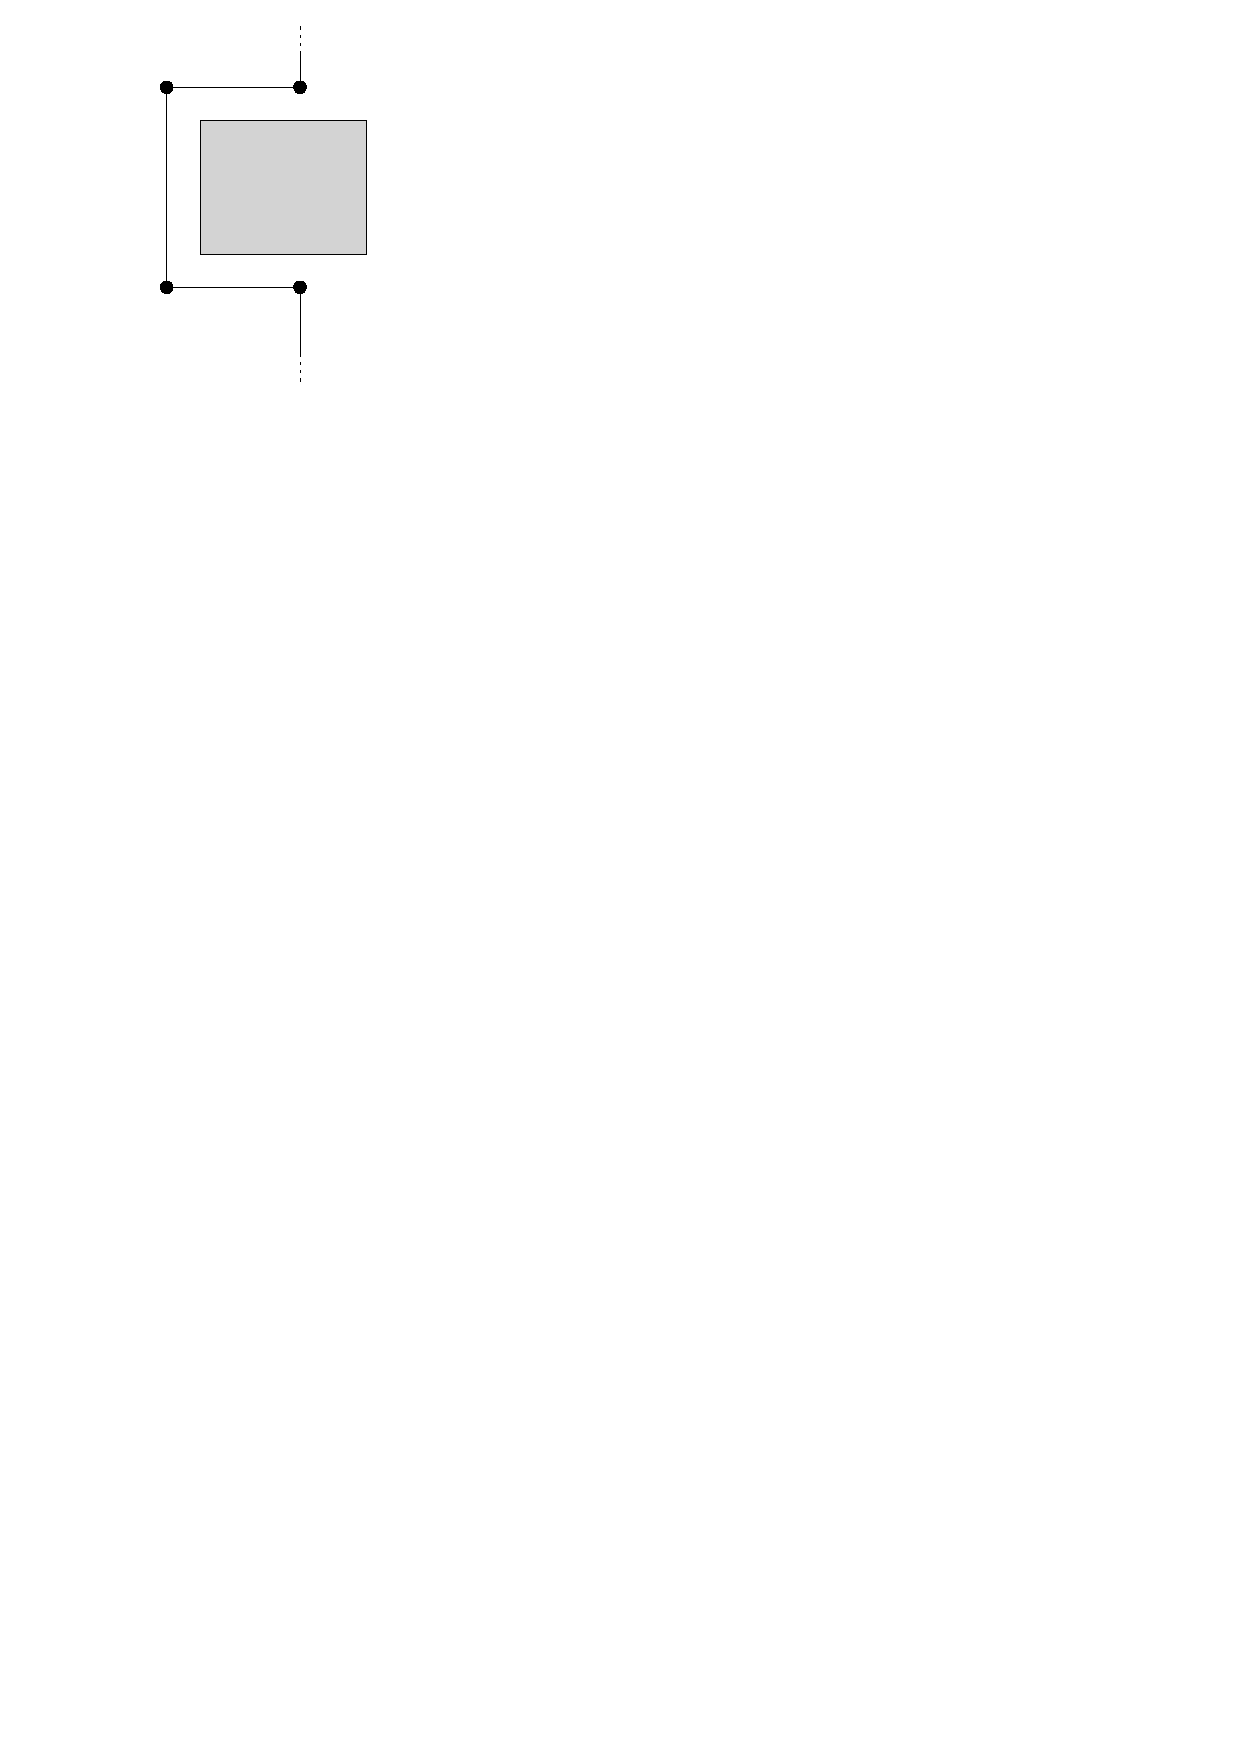
\includegraphics[width=.8\linewidth]{figures/umlauf.pdf}
	\caption{Umlaufung}
	\label{fig:goaround}
\end{minipage}%
\begin{minipage}{.8\textwidth}
  \centering
  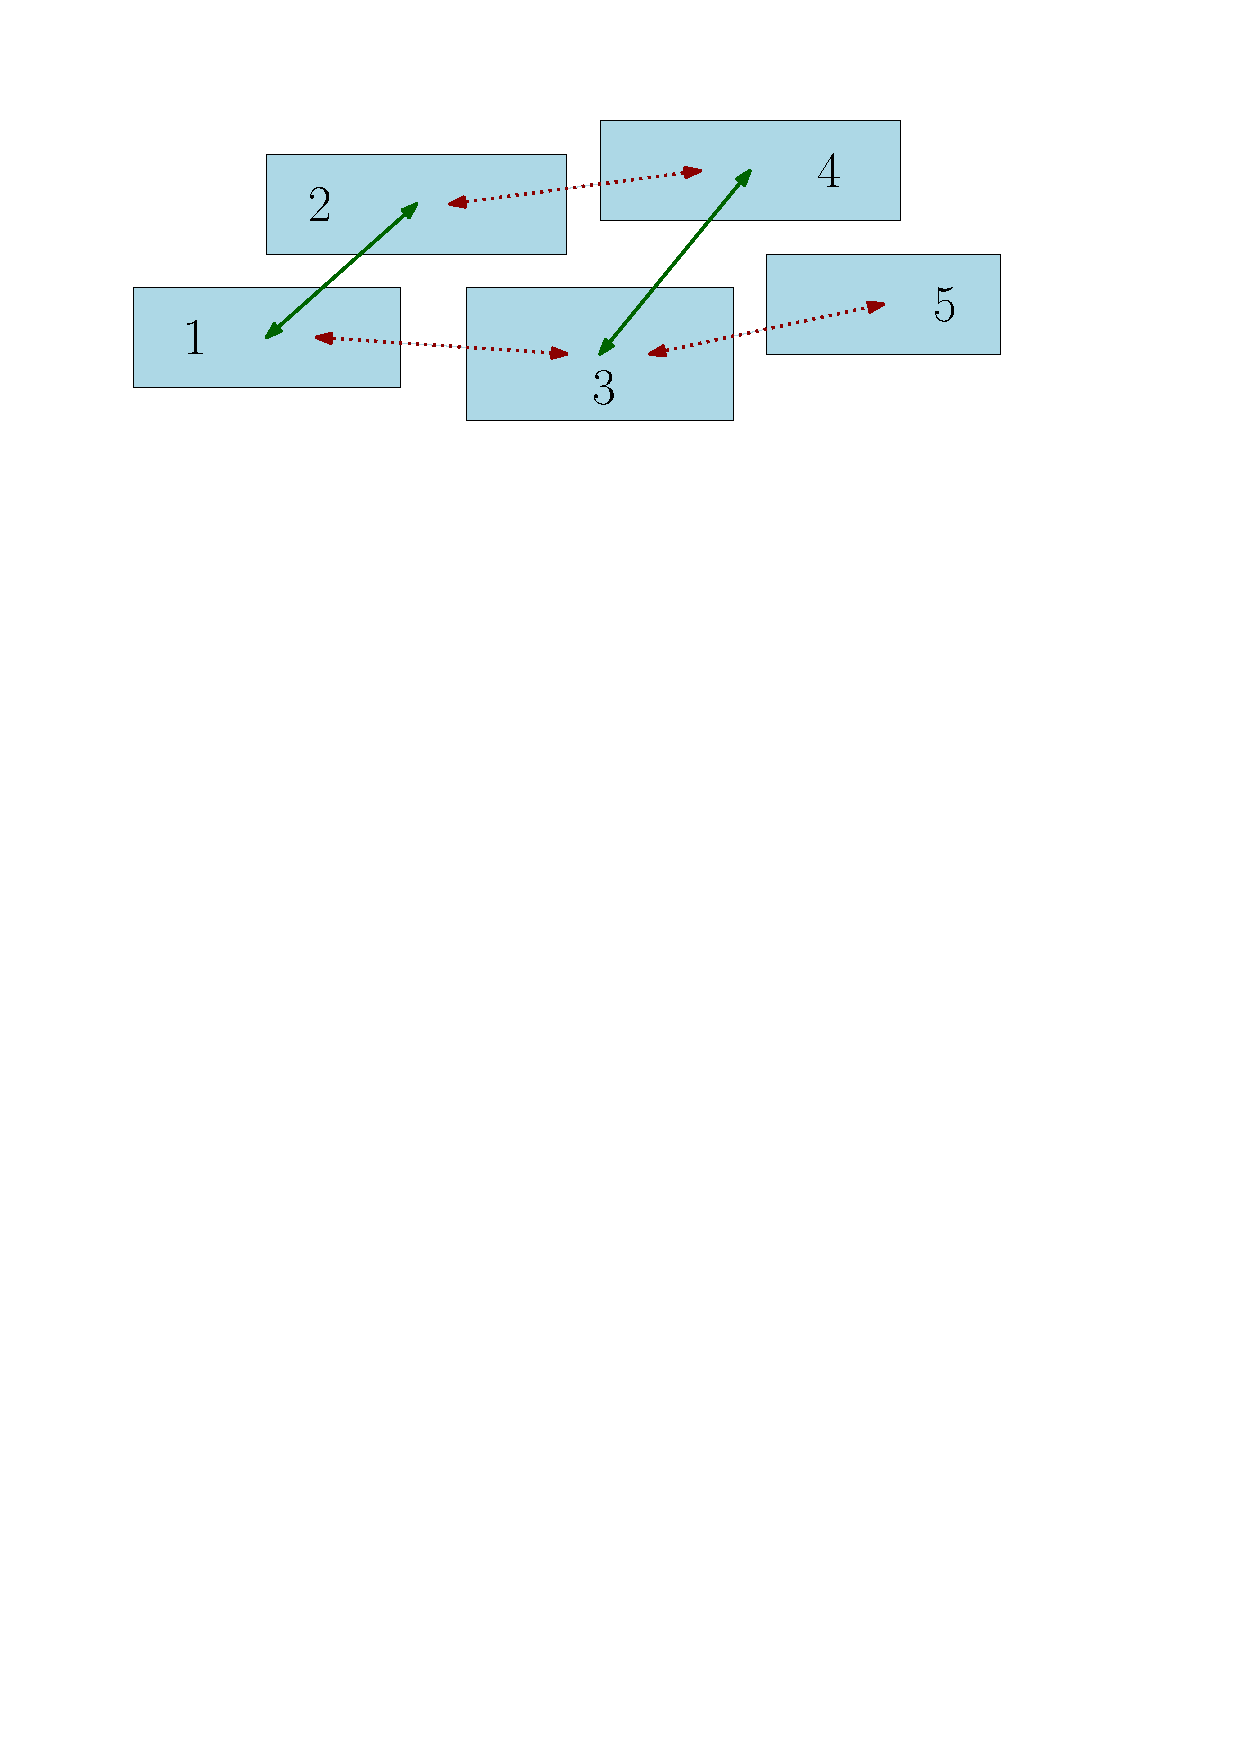
\includegraphics[width=.8\linewidth]{figures/neighbors.pdf}
  \captionof{figure}{Nachbarn}
  \label{fig:neighbors}
\end{minipage}
\end{figure}

Diese Modellierung erlaubt noch keine Knicke zusätzlich zu denen, die schon im Ausgangslayout vorhanden sind. Dies ließe sich umsetzen, indem auf jedem Abschnitt einer Kante zusätzliche Pseudoknicke eingefügt werden, die vom ILP dann genutzt werden können. Zur Knickminimierung ist es hilfreich, die Anzahl der genutzten Pseudoknicke in die Optimierungsfunktion mit aufzunehmen. Es bietet sich an, pro Abschnitt $4$ solcher Pseudoknicke einzufügen, da mit $4$ Knicken in jedem Fall ein Knoten umlaufen werden kann, wie in Abbildung \ref{fig:goaround} zu sehen. Sollten für ein optimales Ergebnis mehr als $4$ zusätzliche Knicke auf einem Kantenabschnitt benötigt werden, so ist eine Lösung ähnlich der in Abschnitt \ref{sub:impl:opt} für die Bedingungen zur Überlappungsfreiheit vorgestellten denkbar: Stellt man nach der Lösung des ILPs fest, dass alle Pseudoknicke auf einem Abschnitt verwendet wurden, so fügt man in die neu entstandenen Abschnitte wiederum je $4$ Pseudoknicke ein und lässt das ILP erneut lösen.

Offensichtlich steigert diese Art Kantenroutings zu betrachten die Komplexität des ILPs noch einmal beträchtlich. Wir haben daher Zweifel daran, dass dies in der Praxis eine nützliche Erweiterung der vorgestellten ILPs ist.


\subsection{Implementation}

Für dieses Seminar haben wir einen Prototypen, der die Implementierung eines der von uns vorgeschlagenen Integer Linear Programs mit einem Editor-Frontend vereint, entwickelt. Diesen möchten wir im Folgenden vorstellen.

\subsection{User Interface}

In diesem Abschnitt wird die grafische Oberfläche, welche Teil des Prototypen ist, mit ihren
Funktionalitäten vorgestellt. Außerdem wird die Bedeutung für einen eigenen Editor im
Rahmen des Seminars erläutert.

\subsubsection{Beschreibung}

Die GUI ist eine Webanwendung, welche mit Javascript programmiert wurde. Hierzu wurden
die Javascript-Bibliotheken Cytoscape.js\cite{cytoscape} und Angular.js\cite{angularjs} benutzt. Cytoscape.js bietet bereits
Funktionalitäten, um einen Graphen darzustellen und zu manipulieren. Angular.js wurde als
Javascript Framework benutzt, um die Interaktion mit HTML und Javascript zu erleichtern.
Ansonsten wurde reines Javascript benutzt, um die weiteren Features zu implementieren.

Da diese Arbeit sich auf das inkrementelle Einfügen von Knoten fokussiert, wurde der Editor
mit einer Funktion ausgestattet, welche es erlaubt, einen Knoten lediglich mit ein paar
Mausklicks einzufügen und die Größe festlegen zu können. Es wird verhindert, dass ein neu
eingefügter Knoten mit einem bestehenden Knoten überlappt, indem für den neuen Knoten
genug Platz geschaffen wird. Der Algorithmus um Platz zu schaffen unterstützt die vier
folgenden Modi:

\begin{itemize}
	\item es wird Platz gemacht, indem alle Knoten in eine der vier orthogonalen Richtungen
verschoben werden, damit unmittelbar links, rechts, oberhalb und unterhalb von dem
neuen Knoten kein anderer Knoten sich befindet. Alle Knoten, die in die gleiche
Richtung verschoben werden, werden um den gleichen Betrag verschoben. Dieser
Betrag wird so bestimmt, dass alle Knoten einen minimalen Abstand von dem
eingefügten Knoten einhalten.
	\item der erste Modus aber es wird nur links und rechts Platz gemacht.
	\item der erste Modus aber es wird nur oben und unten Platz gemacht.
	\item die Knoten werden um den gleichen Betrag nach außen verschoben, damit kein
anderer Knoten mit dem Neuen überlappt
\end{itemize}

In jedem Modus wird ein Mindestabstand zwischen dem neu eingefügten Knoten und allen
anderen eingehalten. Somit kommt es zu keinen Überlappungen der Knoten, die zu nah
beieinander sind. Abhängig vom Modus der gerade aktiv ist zeigt die GUI ein entsprechendes
Overlay um anzuzeigen, wo überall Platz gemacht wird. Nachdem ein Knoten mit einem der
vier Modi eingefügt wurde, kann dessen Größe festgelegt werden. Anschließend hat der
Benutzer die Möglichkeit über einen Button das Layout des Graphen anzupassen. Somit wird
der Platz, der vorher gemacht wurde, wieder minimiert, wobei versucht wird, gewisse
Layoutbedingungen nicht zu verletzen (die wird näher in FIXME beschrieben).
Des Weiteren zeigt jeder Knoten einen Titel und eine Beschreibung an. Somit können
Informationen von Thesen und Argumenten in den Knoten angezeigt werden. Dies ist eine
grundlegende Anforderung an eine Argumentkarte.

Außerdem können Knoten horizontal sowie vertikal auf einer Linie angeordnet werden. Dies
hilft dem Benutzer, den Graphen nach seinen Bedürfnissen zu gestalten. Hier können
verschiedene Funktionen genutzt werden, um neue Position der Knoten zu berechnen. In
dem Prototypen wird der Mittelwert der $x$- oder $y$- Koordinate berechnet und als neue Position
der auszurichtenden Knoten benutzt. Eine weitere Funktion könnte die Knoten an dem zuletzt
markierten Knoten ausrichten oder an einem Knoten ausrichten, den man explizit auswählt.
Da es sich nur um einen Prototypen handelt wurden diese Funktionen jedoch nicht
implementiert.

Die letzte wichtige Funktion ist das Importieren von \textit{.graphml} Dateien. Somit können
Argumentkarten aus dem Argunet-Editor importiert werden. Dies erlaubt ein schnelles Testen
der Algorithmen. Es werden Position und Größe der Knoten, Kanten zwischen den Knoten
und die Beschriftung der Knoten importiert. Falls man ein orthogonales Kantenrouting
implementiert hätte, könnte man hier auch noch die Position der Knicke auf den Kanten
importieren, falls diese in der \textit{.graphml}-Datei vorhanden sind.

\subsubsection{Bedeutung für das Seminar}

Die Anforderung der Philosophiestudenten war, dass der Graph sich nur wenig ändern sollte,
wenn ein Knoten eingefügt wird. Die verschiedenen Modi dienen dazu, dass der Benutzer
entscheiden kann, wie viel sich im Graphen ändert. Hier muss angemerkt werden, dass nur
der erste Modus garantieren kann, dass sich orthogonale Kanten nicht überlappen würden.
Da diese Arbeit sich jedoch ausschließlich auf die Position der Knoten bezieht und die Kanten
ausklammert, wird dieses Problem nicht weiter diskutiert.

Der anschließende Layoutalgorithmus versucht dann so weit es geht das ursprüngliche
Layout wieder herzustellen. Wie ähnlich der Graph nach dem Einfügen des Knoten aussieht,
hängt stark von der Position und der Größe des neuen Knoten ab. Die zusätzliche
Ausrichtfunktion dient dazu, dass der Benutzer in das Layout eingreifen kann, und noch mehr
mitbestimmen kann wie das endgültige Layout aussieht.

Diese beiden Funktionen sind sinnvoll, da der Benutzer, welcher eine Argumentkarte erstellt,
meistens bereits weiß, wie die Knoten angeordnet werden sollen. Insbesondere weiß der
Benutzer auch wie ein neu eingefügter Knoten positioniert werden soll. Der Benutzer ist
jedoch nicht darauf angewiesen diese Layoutfunktionen zu benutzen. Ohne eine Anpassung
vom Benutzer versucht der ILP-Algorithmus eine optimale (und somit in den meisten Fällen
eine für den Benutzer wünschenswerte) Lösung zu finden.
 Die GUI bietet dem Benutzer Funktionen um schnell einen Graphen inkrementell aufzubauen
und zugleich hat er die Freiheit selbst mit zu entscheiden, wie er den Graphen gestaltet.



\subsection{Backend}

Das Backend hat vor allem die Aufgabe, nach einer erfolgten Einfügung ein neues Layout zu berechnen, welches die zu Beginn dieser Arbeit vorgestellte Optimierungsfunktion \ref{eqn:opt:complete} in gewissem Rahmen optimiert. Hierfür haben wir das in Abschnitt \ref{sub:ilp:2} vorgestellte ILP, das Vertauschungen von Knoten in begrenztem Maße zulässt, mit einigen Anpassungen implementiert.

Beim Backend haben wir auf eine Implementierung in Python unter Zuhilfenahme des Django-Webframeworks\cite{django} gesetzt, die mit der GUI über Ajax kommuniziert. Für die Lösung des ILPs kommt Gurobi\cite{gurobi} zum Einsatz.

\subsubsection{Abweichungen vom beschriebenen ILP}
\label{sub:impl:opt}

Zunächst haben wir wie in Abschnitt \ref{sub:ilp:2} schon angedeutet versucht, die Anzahl der Bedingungen, die für Überlappungsfreiheit sorgen werden, auf eine sub-quadratische Anzahl zu senken. Eine hilfreiche Beobachtung ist hier, dass viele dieser Bedingungen nicht benötigt werden, da die entsprechenden Knoten aufgrund des Abstands zueinander im Ausgangslayout sowieso nicht überlappen werden. Wir fügen daher dem ILP anfangs nur entsprechende Bedingungen für adjazente Knoten hinzu, und werden weitere Bedingungen nur dann ins ILP aufnehmen, wenn sie benötigt werden. Unser erster Ansatz war hier, die Callback-Funktionalität von Gurobi zu nutzen. Dies erwies sich allerdings als unnötig aufwändig, da diese Callbacks teilweise nur unter sehr speziellen Bedingungen aufgerufen werden. Eine einfachere und effiziente Lösung ist es, nach Lösung des ILPs durch Gurobi alle Knoten auf Überlappungen zu testen, bei Bedarf neue Bedingungen einzufügen und das bereits gelöste, aber veränderte Modell von Gurobi erneut lösen zu lassen. Im Normalfall ist eine neue Lösung, die die zusätzlichen Bedingungen berücksichtigt, dann in sehr kurzer Zeit gefunden. Dies wiederholen wir so lange, bis keine Überlappungen mehr auftreten. In unseren Tests sind im Normalfall nicht mehr als eine oder zwei Wiederholungen nötig gewesen.

Eine weitere Besonderheit ist, dass wir für die Vektor-Vektor-Abstände, wie sie z.B. in der Optimierungsfunktion \ref{eqn:opt:complete} vorkommen, die 1-Norm statt der intuitiv vielleicht sinnvolleren 2-Norm verwendet haben. Dies hat den Grund, dass sich die 2-Norm in einem Integer \textit{Linear} Program nicht abbilden lässt. Es wäre an dieser Stelle zwar möglich ein Integer \textit{Quadratic} Program stattdessen aufzustellen (und von Gurobi lösen zu lassen), allerdings wollten wir die Komplexität zunächst auf ein ILP beschränken.

Des Weiteren haben wir zusätzlich eine Klasse von Bedingungen eingebaut, die es ermöglicht, mehrere Knoten auf dieselbe $x$- oder $y$-Koordinate zu zwingen. Dies ist vor allem auf den in Abschnitt \ref{sub:tasks} angesprochenen Wunsch zurückzuführen, mehrere Knoten aneinander "`ausrichten"' zu können.

Eine weitere Optimierung, die die Zeit, die zum Lösen des Systems stark senkt, ist, dass wir die Positionen aller Knoten im Ausgangslayout an die von Gurobi verwendeten Heuristiken zum Finden einer Startlösung übergeben.

\subsection{Ergebnisse}

Wir haben den von uns entwickelten Prototypen mit einigen bereitgestellten GraphML-Dateien getestet. Die Instanzen hatten eher kleine Größen von ca. 20 Knoten. Auf diesen Instanzen wurde das ILP von Gurobi nahezu in Echtzeit gelöst.

\begin{figure}
	\begin{center}
		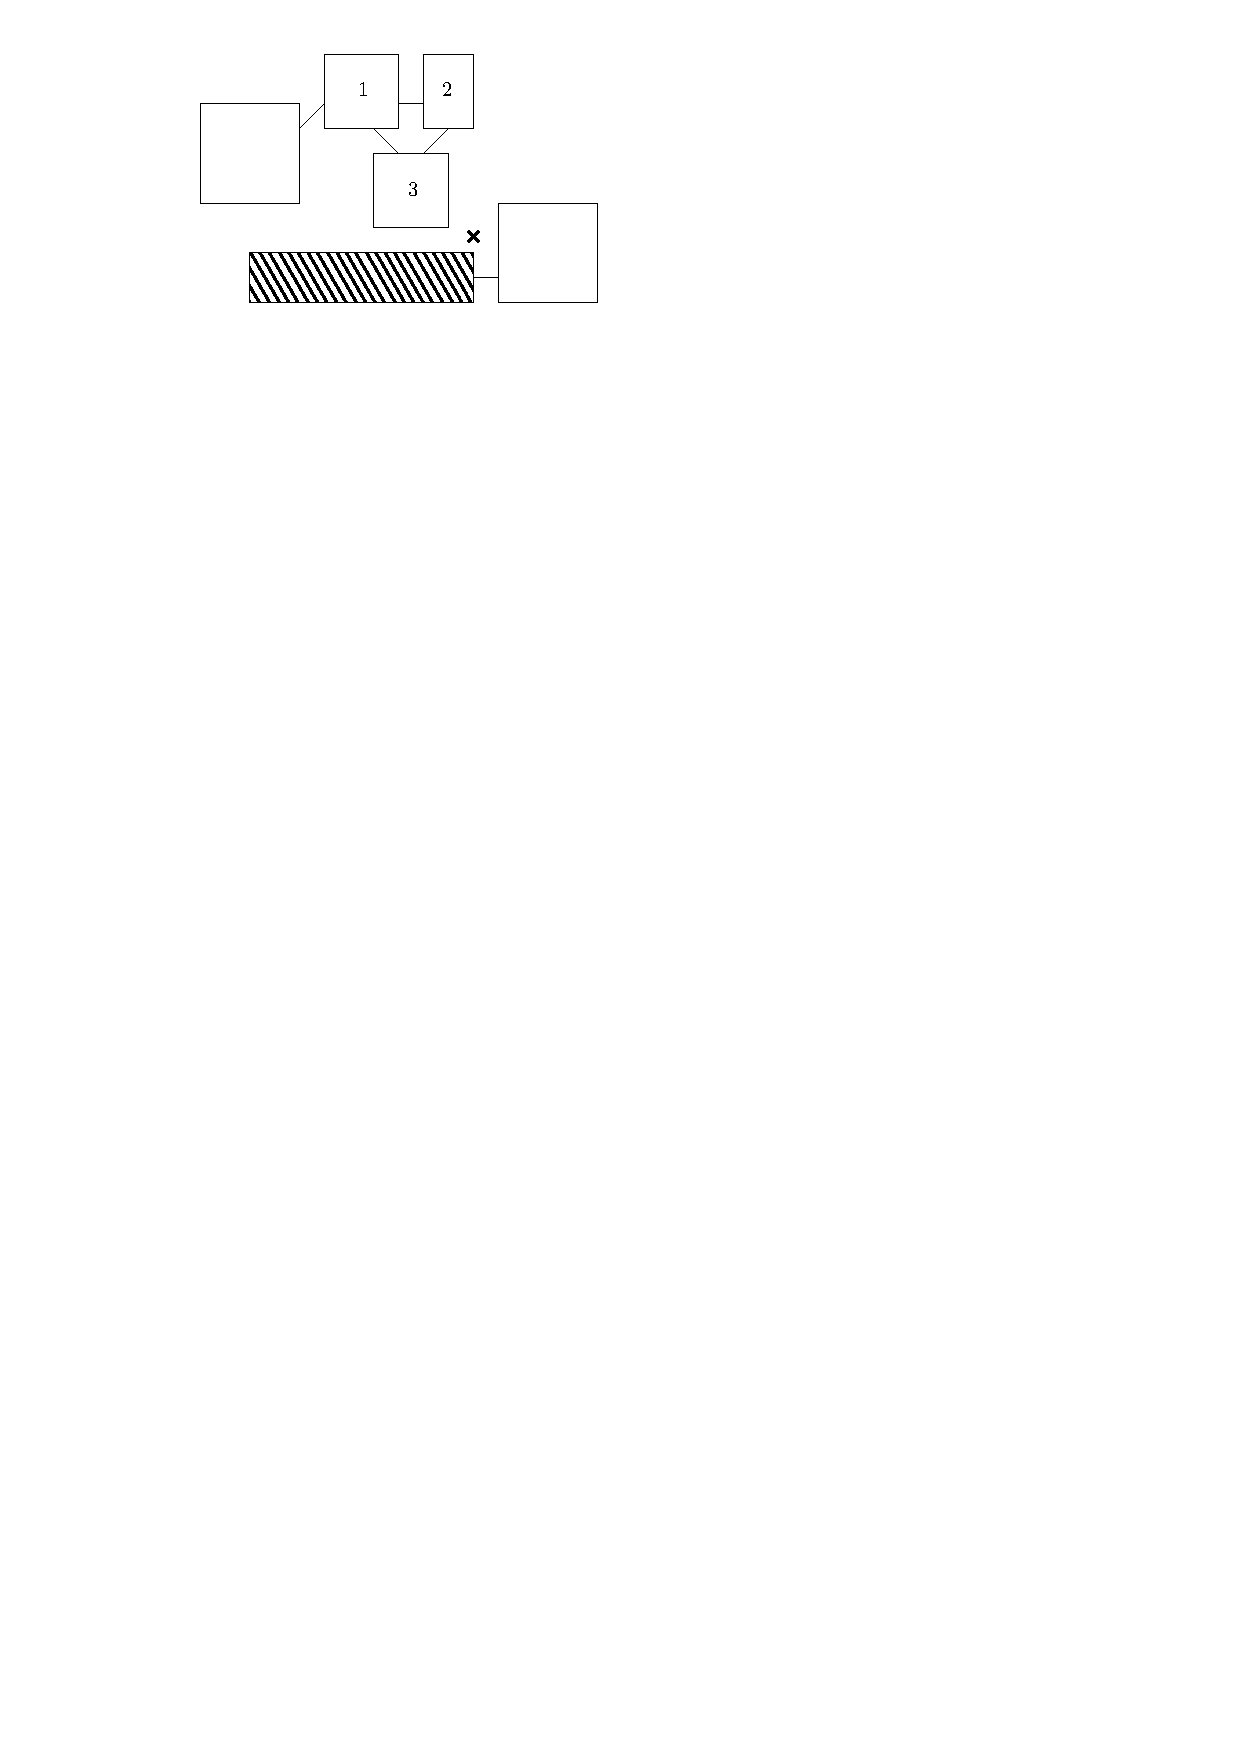
\includegraphics{figures/order.pdf}
		\caption{Problematische Einfügung}
		\label{fig:order-too-strict}
	\end{center}
\end{figure}

Die wichtigste Beobachtung ist, dass die Einschränkung, nur direkt benachbarte Paare von Knoten tauschen zu dürfen, für realistische Instanzgrößen unpraktikabel ist. Am Beispiel von Abbildung \ref{fig:order-too-strict} wird dies deutlich: Der schraffierte Knoten sollte an der Position, die durch das Kreuz angezeigt wird, eingefügt werden. Die Position, an der der schraffierte Knoten jetzt gezeichnet wurde, wäre vermutlich eine gute Wahl. Um hier platziert zu werden, müsste er allerdings (relativ zu der Position des Kreuzes und der links-oberen Ecken der Knoten) in der horizontalen Reihenfolge die Positionen mit den Knoten $1, 2$ und $3$ tauschen, was in diesem eingeschränkten Modell nicht möglich ist. Dieses Problem wird umso ausgeprägter, je größer die Instanzen werden. TODO mehr dazu

Beobachtet haben wir außerdem, dass der neu eingefügte Knoten unserem Gefühl nach häufig zu weit von der Position, an der man ihn hat einfügen wollen, platziert wurde. Außerdem wurde unserem Gefühl nach die Möglichkeit der Skalierung gegenüber der Verschiebung von Knoten (siehe Abschnitt \ref{par:scale}) zu intensiv genutzt wurde. Dies ist zurückzuführen auf die Wahl der Konstanten $\alpha, \beta$ und $\gamma$ in der Optimierungsfunktion \ref{eqn:opt:complete}.



TODO größere Instanzen?


%%% conclusion.tex
%%

%% ==================
%\chapter{Conclusion}
%\label{ch:conclusion}
%% ==================

TODO besserer Name?

\subsection{Weitere Schritte}

\subsubsection{Größere Instanzen}
\label{sub:next:bigger}

Außerhalb des Rahmens dieses Seminars war es leider, eine genauere Evaluation des implementierten ILPs, insbesondere an größeren Instanzen, vorzunehmen. Hier wäre es vermutlich zunächst ratsam, einen Weg zu finden, automatisiert beliebig große Beispiele für Argumentkarten zu generieren. Um solche Beispiele automatisiert erzeugen zu können, wäre es zunächst notwendig, die Eigenschaften zu identifizieren, die eine Argumentkarte ausmachen. Vermutlich wäre dies auch für sich genommen eine interessante Fragestellung.

Blah. Nicht-orthogonale Kanten im ILP.



%% --------------------
%% |   Bibliography   |
%% --------------------

\cleardoublepage
\phantomsection
\addcontentsline{toc}{chapter}{\bibname}

\iflanguage{english}
{\bibliographystyle{alpha}}
{\bibliographystyle{babalpha-fl}} % german style

\bibliography{references}


%% ----------------
%% |   Appendix   |
%% ----------------

%\cleardoublepage
%%% appendix.tex
%%

%% ==============================
%\chapter{Appendix}
%\label{ch:Appendix}
%% ==============================

\appendix

% \iflanguage{english}
% {\addchap{Appendix}}	% english style
% {\addchap{Anhang}}	% german style


\section{Appendix Section 1}
\label{appendix1}

\begin{figure} [ht]
  \centering
   ein Bild
  \caption{A figure}
  \label{fig:BPMNBeispiela}
\end{figure}



\end{document}
